\documentclass[sisc-eikonal.tex]{subfiles}

\begin{document}

\section{Ordered line integral methods for the eikonal equation}

The fast marching method discretizes the eikonal equation,
\cref{eq:eikonal}, and solves this discretization in an upwind fashion
to compute $\hat{U}$. The ordered line integral method locally and
approximately minimizes the minimum action integral of
\cref{eq:eikonal}:
\begin{equation}
  \label{eq:action-functional}
  \hat{u} = \min_{\alpha} \set{u_0 + \int_\alpha s(x) dl},
\end{equation}
where $\alpha$ is a ray parametrized by arc length, $\hat{x}$ is a
target point, $\hat{u} = u(\hat{x})$, and $u_0 = u(\alpha(0))$ (see
\cref{sec:minimum-action-integral} for a derivation of
\cref{eq:action-functional}). By constrast, Lagrangian methods (i.e.,
raytracing methods) trace a bundle of rays from a common locus by
integrating \cref{eq:action-functional} for different initial
conditions. In this section, we describe our approach to discretizing
and approximately minimizing \cref{eq:action-functional}. As we
mentioned in \cref{ssec:dijkstra-like}, to compute
$\hat{U} = U(\hat{p})$ in \cref{enum:update-U} of
\cref{alg:dijkstra-like}, we need to approximately minimize several
instances of \cref{eq:action-functional}; details of this procedure
will be discussed in \cref{sec:implementation}. In this section, we
focus on a single instance of the discretized version of
\cref{eq:action-functional}. We first present notation, derive
prelimary results, describe the different quadrature rules we use,
detail useful exact solutions to the approximate minimization of
\cref{eq:action-functional}, and present theoretical results.

\begin{figure}
  \centering
  \begin{subfigure}{.4\textwidth}
    \centering
    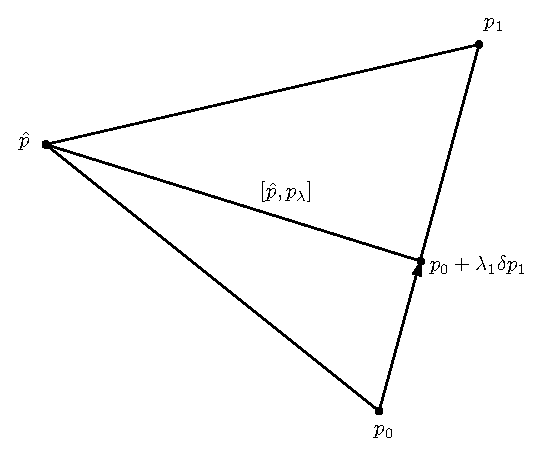
\includegraphics[width=\linewidth]{tri-diagram.eps}
    \caption{An example with $d = 1$ (a triangle
      update).}\label{fig:tri-diagram}
  \end{subfigure}%
  \begin{subfigure}{.4\textwidth}
    \centering
    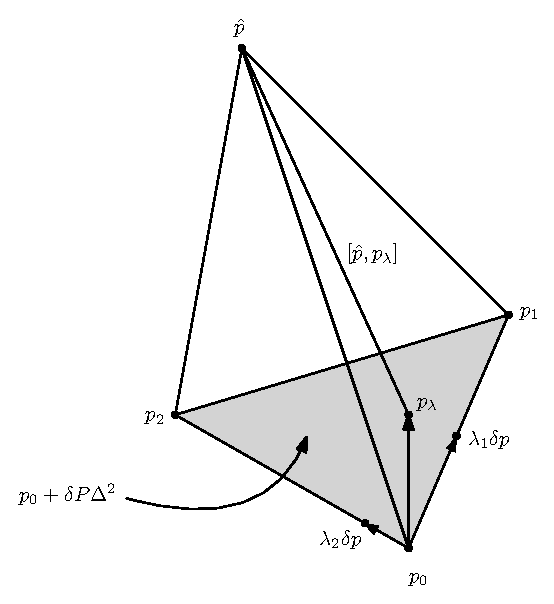
\includegraphics[width=\linewidth]{simplex-diagram.eps}
    \caption{An example with $d = 2$ (a tetrahedron
      update).}\label{fig:tetra-diagram}
  \end{subfigure}
  \caption{Characteristics emanate from the set
    $p_0 + \delta P \Delta^d = \set{p_0 + \lambda_1 \delta p_1 +
      \cdots + \lambda_d \delta p_d}$, which approximates the front of
    the numerical solution.}\label{fig:simplex-diagrams}
\end{figure}

\subsection{Notation}

When minimizing the action functional, we minimize a line integral
whose path is constrained to lie in a simplex (lines, triangles, and
tetrahedra in 2D and 3D). This is depicted in
\cref{fig:simplex-diagrams}; in particular, the range of
$\left. \alpha \right|_{[0, 1]}$ is $[\hat{p}, p_{\lambda}]$. Since we
solve \cref{eq:eikonal} on a regular grid, there are only a small
number of distinct simplices that we need to treat in our
implementation, each with fixed geometry but varying data. It ends up
being beneficial to rescale their vertices to $\mathbb{Z}^n$ and
translate each so that $\hat{p} = 0$.

Let $n \geq 2$ be an integer and assume
$d \in \set{0, \hdots, n - 1}$. Let
$p_0, \hdots, p_d \in \Z^n \backslash \set{0}$ be linearly
independent. Together with $\hat{p} = 0$, these vectors are the
vertices of a simplex with affine dimension $d + 1$ (the affine
dimension of $\set{p_0, \hdots, p_d}$ is $d$). In this work, we will
also only consider vectors $p_i$ for which $\norm{p_i}_\infty =
1$. For each $i = 0, \hdots, d$, we also define $x_i$ to be the
preimage of $p_i$ before scaling and translation is performed (i.e.,
each $x_i$ lies in $h \Z^n$). The numerical solution $U$ and the
slowness function $s$ are evaluated at the points $x_i$; we write
$U_i = U(x_i)$ and $s_i = s(x_i)$. For fixed $n$, it will be necessary
to solve minimization problems corresponding to simplices of all
dimensions up to and including $n - 1$. We will cover this in more
detail in a later section; presently, we will derive the updates for
general dimension since there is no need to specialize. Along these
lines, unless we have reason to distinguish the dimension $d$ of the
update simplex, we will simply assume that $d = n - 1$.

Next, define the set $\Delta^d$ by:
\begin{equation}
  \Delta^d = \set{(\lambda_1, \hdots, \lambda_d) : \lambda_i \geq 0 \mbox{ for } i = 1, \hdots, d \mbox{ and } \sum_{i=1}^d \lambda_i \leq 1}.
\end{equation}
For each $\lambda = (\lambda_1, \hdots, \lambda_d) \in \Delta^d$, we
will write $\lambda_0 = 1 - \lambda_1 - \cdots - \lambda_d$. Then,
$\sum_{i=0}^d \lambda_i p_i$ lies in the convex hull of
$\set{p_0, \hdots, p_d}$. We denote this vector by
$p_\lambda$. Defining $\delta p_i = p_i - p_0$, we can also write
$p_\lambda = p_0 + \sum_{i=1}^d \lambda_i \delta p_i$ and define the
matrix:
\begin{equation}
  \delta P = \begin{pmatrix} \delta p_1 & \cdots & \delta p_d \end{pmatrix} \in \R^{n \times d},
\end{equation}
so that we can write $p_\lambda = \delta P \lambda + p_0$. Along the
same lines, $U_\lambda = U_0 + \delta U^\top \lambda$, where
$\delta U_i = U_i - U_0$; we also define $\delta s_i = s_i - s_0$, and
vectorial versions of each of these, $\delta U$ and $\delta
s$. Observe that the role of the points $x_i$ is obscured here: each
update can be parametrized by the vectors $\set{p_i}$ and the problem
data $(U, s, h)$. We also mention here that although the slowness
function $s$ may be available to us in analytic form, we assume that
it is only available on the nodes in $\calG$ to reflect the realities
of likely use cases.

\subsection{Quadrature}\label{ssec:quadrature}

To minimize \cref{eq:action-functional}, we assume that $\alpha$ is a
line segment parametrized by arc length and then apply several
different one-point quadrature rules to the resulting integral.

If $\alpha$ is a line segment connecting $p_\lambda$ and
$\hat{p} = 0$, then:
\begin{equation}
  \label{eq:action-functional-line-segment}
  \hat{U} = U(\hat{p}) = \min_{\lambda \in \Delta^d} \set{U_\lambda + h \int_{[p_\lambda, 0]} s(\alpha(t))dt}.
\end{equation}
We consider two approximations to \cref{eq:action-functional-line-segment}: the
difference between the two pertains to the way we incorporate the
slowness function $s$. Let $\theta \in [0, 1]$ and define
$l_\lambda = \norm{p_\lambda}_2$. For $\theta$ such that
$0 \leq \theta \leq 1$, we define:
\begin{align}
  F_0(\lambda) = F_0^\theta(\lambda) &= U_\lambda + s^{\theta} h l_\lambda := U_\lambda + \squareb{(1-\theta)\hat{s} + \frac{\theta}{d + 1} \sum_{i=0}^d s_i} h l_\lambda, \label{eq:f0-definition} \\
  F_1(\lambda) = F_1^\theta(\lambda) &= U_\lambda + s^{\theta}_\lambda h l_\lambda := U_\lambda + \squareb{(1-\theta)\hat{s} + \theta s_\lambda} h l_\lambda,
\end{align}
where we typically omit the superscript in $F_i^\theta$. We will
primarily concern ourselves with $F_0$ and $F_1$ for $\theta = 0$ and
$\theta = \nicefrac{1}{2}$. If $\theta = 0$, then $F_0 \equiv F_1$, so
we define a single quadrature rule to capture this case, called
\texttt{rhr}. If $\theta = \nicefrac{1}{2}$, then $F_0 \neq F_1$ in
general, leading us to define a separate midpoint quadrature rule for
each of $F_0$ and $F_1$, named \texttt{mp0} and \texttt{mp1},
respectively. The case of \texttt{mp0} requires special care and is
handled in \cref{ssec:validation}.

\begin{figure}[t]
  \centering
  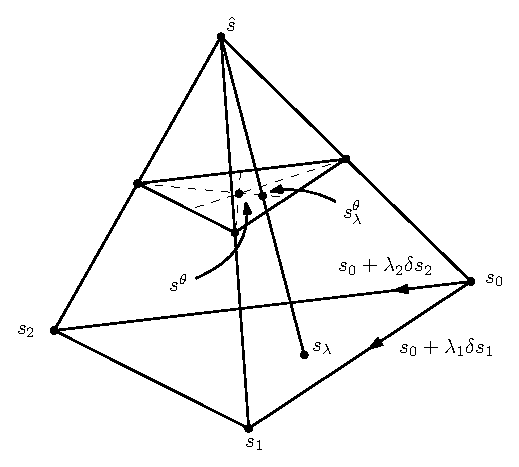
\includegraphics{slowness-tetra.eps}
  \caption{A depiction of the different quantities related to
    $s^{\theta}$ and $s^{\theta}_\lambda$ for the case of $d = 2$, a
    tetrahedron update. Both of $s^\theta$ and $s^\theta_\lambda$ live
    on the $\theta$-section of the simplex
    $\conv \set{\hat{p}, p_0, p_1, p_2}$. The function
    $s^\theta_\lambda$ is a linear combination of $\hat{s}, s_0, s_1$,
    and $s_2$; the value $s^\theta$ is $s^\theta_\lambda$ evaluated at
    the centroid of the $\theta$-section.}
\end{figure}

\subsection{The minimization problem}

With $F_0$ and $F_1$ so defined, we can pose our minimization problem
which approximately solves
\cref{eq:action-functional,eq:action-functional-line-segment} to
compute $\hat{U}$ for a fixed update simplex:
\begin{equation}
  \label{eq:constrained-minimization}
  \hat{U} = \min_{\lambda \in \Delta^d} F_i(\lambda).
\end{equation}
This is a nonlinear, constrained optimization problem with linear
inequality constraints and no equality constraints. We will find the
gradient and Hessian of $F_0$ and $F_1$ to be useful in our algorithms
and analysis. These quantities are easy to compute, but we have found
a particular form for them to be appropriate. We compute these
quantities in the following two lemmas.

\begin{lemma}\label{lemma:F0-grad-and-Hess}
  The gradient and Hessian of $F_0(\lambda; \theta)$ satisfy:
  \begin{align}
    \nabla F_0(\lambda) &= \delta U + s^{\theta} h \delta P^\top \nu_\lambda,\label{eq:F0-grad} \\
    \nabla^2 F_0(\lambda) &= \frac{s^{\theta} h}{l_\lambda} \delta P^\top \calP^\perp_{p_\lambda} \delta P,
  \end{align}
  where $\nu_\lambda = p_\lambda/l_\lambda$,
  $\calP_{p_\lambda} = \nu_\lambda \nu_\lambda^\top$ denotes the
  orthogonal projector onto $\operatorname{span}(p_\lambda)$ and
  $\calP_{p_\lambda}^\perp = I - \nu_\lambda \nu_\lambda^\top$ is the
  orthogonal projector onto $\operatorname{span}(p_\lambda)^\perp$.
\end{lemma}

\begin{lemma}\label{lemma:F1-grad-and-Hess}
  The gradient and Hessian of $F_1(\lambda; \theta)$ satisfy:
  \begin{align}
    \nabla F_1(\lambda) &= \delta U + \theta h l_\lambda \delta s + s^{\theta}_\lambda h \delta P^\top \nu_\lambda, \\
    \nabla^2 F_1(\lambda) &= \set{\delta P^\top \nu_\lambda, \theta h \delta s} + \frac{s^\theta_\lambda h}{l_\lambda} \delta P^\top \calP^\perp_{p_\lambda} \delta P, \label{eq:hess-F1}
  \end{align}
  where $\set{a, b} = ab^\top + ba^\top$ is the anticommutator of two
  vectors.
\end{lemma}

Since our task will be to minimize nonlinear functions $F_0$ and $F_1$
over a convex set, $\Delta^n$, we are interested in determining
whether $F_0$ and $F_1$ are convex themselves. The next two lemmas
address this point. There is some question as to whether $F_0$ and
$F_1$ are strictly convex or just convex. This relates to the
definiteness of their Hessians, computed above. The conditions that
$p_0, \hdots, p_d$ span a nondegenerate simplex---i.e, $\set{p_i}$ is
linearly independent---and that $\smin = \min_\calG s > 0$ are
sufficient in this case.

\begin{lemma}\label{lemma:dPt-cprojp-dP-pd}
  Let $\set{p_i}$ form a nondegenerate update simplex together with
  $\hat{p}$ and assume that $\smin > 0$. Then, $\nabla^2 F_0$ is
  positive definite and $F_0$ is strictly convex.
\end{lemma}

For $F_1$, we can only obtain convexity (let alone strict convexity)
as $h \to 0$. For large enough $h$, we will encounter nonconvex
updates. To obtain convexity, we need to stipulate that the slowness
function $s$ be modestly Lipschitz continuous on $\Omega$.

\begin{lemma}\label{lemma:F-strictly-convex}
  Again, assume that the update simplex is nondegenerate and $\smin >
  0$. Additionally, assume that
  $s$ is Lipschitz continuous with Lipschitz constant $K \leq
  Cn^{-1/2}$ on $\Omega$, for some constant $C > 0$. Then, $\nabla^2
  F_1$ is positive definite as $h \to 0$; hence,
  $F_1$ is strictly convex as $h \to 0$.
\end{lemma}

In practice, we have found that essentially all \texttt{mp1} updates
become strictly convex quite rapidly as $h \to 0$, and there is no
issue of convergence. Despite this, our solvers are designed to be
robust to this problem. See \cref{sec:implementation}.

\subsection{Validation of \texttt{mp0}}\label{ssec:validation}

If we consider an update simplex defined by the nodes
$p_0, \hdots, p_{n-1}$, each subset of these nodes defines another
valid update simplex. For example, consider the three triangle updates
forming the boundary of a single tetrahedron update. We expect the
values of $F_i$ to be the same when defined on one or another update
simplex, and to be continuous as we transfer between simplices that
share a common boundary. For $F_1$ this is the case, but for $F_0$
with $\theta \neq 0$, the function $F_0$ may not be well-defined at
boundaries or continuous from simplex to simplex. This problem leads
to inconsistent and divergent solvers. A heuristic fix is to first
minimize \cref{eq:constrained-minimization} for $F_0$ with nonzero
$\theta$ to obtain the minimizing argument $\lambda^*_0$, then set
$\hat{U} = F_1(\lambda_0^*)$; i.e., we replace $F_0$ with $F_1$ for
the purposes of evaluation.

If we apply Newton's method to the minimization of $F_1^\theta$,
starting at $\lambda_0^*$ and letting $\lambda_1^*$ denote the optimum
of \cref{eq:constrained-minimization} where $i = 1$, then we can use
use the attendant theory of Newton's method to prove the following
result which bounds the distance between $\lambda_0^*$ and
$\lambda_1^*$, thereby bounding the error incurred by \texttt{mp0}
over \texttt{mp1}~\cite{stoer2013introduction}.

\begin{theorem}\label{theorem:mp0-newton}
  Let $h$ be sufficiently small so that $F_1$ is strictly convex by
  \cref{lemma:F-strictly-convex}. Then, the error vector
  $\delta\lambda^* = \lambda_1^* - \lambda_0^*$ satisfies
  $\norm{\delta\lambda^*} = O(h)$. Additionally, if we let
  $\lambda_0 = \lambda_0^*$ in the following Newton iteration:
  \begin{equation}
    \label{eq:lam0-iter-to-lam1}
    \lambda_{k+1} \gets \lambda_k - \nabla^2 F_1(\lambda_k)^{-1} \nabla F_1(\lambda_k), \qquad k = 0, 1, \hdots,
  \end{equation}
  then this iteration is well-defined, and converges quadratically to
  $\lambda_1^*$.
\end{theorem}

The proof of \cref{theorem:mp0-newton} relies on some technical
lemmas which are detailed in \cref{app:validation-proofs}. This
theorem immediately implies the following error bound.

\begin{theorem}\label{thm:mp0-error}
  The error incurred by \texttt{mp0} is $O(h^3)$ per update compared
  to \texttt{mp1}; i.e.:
  \begin{equation}
    \label{eq:mp0-error}
    \abs{F_1(\lambda_1^*) - F_1(\lambda_0^*)} = O(h^3).
  \end{equation}
\end{theorem}

This bound is satisfactory in the following way: if we assume that our
domain is spanned along a diameter by $O(N)$ nodes, and that
$h \sim N^{-1}$, then we can anticipate $O(N)$ downwind updates,
starting from $\boundary$ and extending to the boundary of
$\calG$. Accumulating the error over these nodes, we can expect the
maximum pointwise error between a solution to \cref{eq:eikonal}
computed by using \texttt{mp0} and \texttt{mp1} to be $O(h^2)$, which
is dominated by the $O(h)$ discretization error coming from the linear
convergence of the method itself.

Also, note that if we exchange the roles of $F_0$ and $F_1$---i.e., if
we start from $\lambda_1^*$ and perform a Newton iteration on
$\nabla F_0$---we can obtain the foregoing error bound again, and
possibly with less effort. The main reason to start from $\lambda_0^*$
and drive to $\lambda_1^*$ is that it allows us to use \texttt{mp0} to
initialize \texttt{mp1}. For $d = 0, 1$, this is unimportant, but in
higher dimensions especially, minimizing $F_0$ should be
cheaper. Reducing the number of $F_1$ update iterations suggests a
sped-up method with the same accuracy.

\subsection{Exact solution for \texttt{rhr} and \texttt{mp0}}\label{ssec:exact-soln}

Since $F_0$ is strictly convex, $\nabla F_0(\lambda) = 0$ is
sufficient for optimality of $\lambda$. The system of nonlinear
equations defined by $\nabla F_0(\lambda) = 0$ can be solved exactly
without appealing to an iterative solver. Instead, we can compute the
solution from the reduced QR decomposition of $\delta P$ and geometric
consideration of the minimization problem. This is captured by the
following theorem, and the geometry of the problem is depicted in
\cref{fig:f0-exact}.

\begin{theorem}\label{thm:f0-exact}
  Let $\delta P = QR$ be the reduced QR decomposition of $\delta P$;
  i.e., such that
  $Q \in \mathbb{R}^{n \times d}, R \in \mathbb{R}^{d \times d},
  Q^\top Q = I_d$, and such that $R$ is upper triangular. For fixed
  problem data $s^\theta, h$, and $U$, if
  $\lambda^* = \argmin_{\lambda \in \mathbb{R}^n}
  F_0^\theta(\lambda)$, we have:
  \begin{align}
    l_{\lambda^*} &= \sqrt{\frac{p_0^\top {(I - QQ^\top)} p_0}{1 - \norm{R^{-\top} \frac{\delta U}{s^\theta h}}^2}},\label{eq:l-star-expression} \\
    \lambda^* &= -R^{-1} \parens{Q^\top p_0 + l_{\lambda^*} R^{-\top} \frac{\delta U}{s^\theta h}},\label{eq:f0-exact-lambda} \\ 
    \hat{U} &= U_0 + \frac{s^\theta h}{l_{\lambda^*}} p_0^\top p_{\lambda^*}.\label{eq:f0-exact}
  \end{align}
\end{theorem}

\subsection{Equivalence of the upwind finite difference scheme and
  $F_0$}\label{ssec:equivalence}

If we linearly approximate $U$ about $\hat{p}$, then for
$i = 0, \hdots, n - 1$, we find that $\hat{U}$ approximately
satisfies:
\begin{equation}
  \label{eq:finite-differences}
  U_i - \hat{U} = \nabla \hat{U}^\top p_i.
\end{equation}
This finite difference approximation to \cref{eq:eikonal} can be
solved exactly and is a generalization of the upwind finite difference
scheme used by the fast marching method to an unstructured
mesh~\cite{sethian2000fast}. Computing $\hat{U}$ using this
approximation turns out to be equivalent to solving:
\begin{equation}
  \hat{U} = \min_{\lambda \in \Delta^n} F_0(\lambda),
\end{equation}
in a sense made precise by the following theorem.

\begin{theorem}[Equivalence of upwind finite difference scheme and $F_0$]\label{thm:equivalence}
  Let $\hat{U}$ by the finite difference solution and let
  $\hat{U}' = \min_{\lambda \in \R^n} F_0(\lambda)$. Then, $\hat{U}$
  exists if and only if $\|R^{-\top} \delta U\| \leq s^\theta h$
  holds; when this is the case, $\hat{U}$ can be computed from:
  \begin{equation}
    \label{eq:U-finite-diff}
    \hat{U} = U_i - p_i^\top Q R^{-\top} \delta U + \norm{\pmin} \sqrt{{(s^\theta h)}^2 - \norm{R^{-\top} \delta U}^2},
  \end{equation}
  and the following properties hold:
  \begin{enumerate}
  \item The finite difference solution and line integral solution
    coincide: $\hat{U} = \hat{U}'$ can be computed from:
    \begin{equation}
      \label{eq:U-from-Ui-exact}
      \hat{U} = U_i + \frac{s^\theta h}{l_{\lambda^*}} p_i^\top p_{\lambda^*}
    \end{equation}
    where
    $\lambda^* = \argmin_{\lambda \in \R^n}
    F_0(\lambda)$.
  \item The characteristics found by solving the finite difference
    problem and minimizing $F_i$ coincide and are given by
    $[p_{\lambda^*}, \hat{p}] = [p_{\lambda^*}, 0]$.
  \item In either case, the characteristic passes through
    $\conv(p_0, \hdots, p_{n-1})$ if and only if
    $\lambda^* \in \Delta^n$.
  \end{enumerate}
\end{theorem}

\subsection{Causality}\label{ssec:causality}

\hl{\textbf{TODO}}: specifically, why is causality important? Explain
what causality implies, why we're bothering with proving it, and
provide a citation that explains the idea in more depth.

We deal with causality simplex by simplex; hence, we will refer to
update simplices being causal or not. Since we always assume that our
update simplices have been translated so that $\hat{p} = 0$, whether
or not a simplex is causal depends only on the vertices
$p_0, \hdots, p_{n-1}$. We also have causality with respect to $F_0$
and $F_1$.

\begin{definition}
  An update simplex defined by the vectors $p_0, \hdots, p_{n-1}$ is
  \emph{causal} if, for any problem data, $\hat{U} \geq \max_i U_i$
  holds, where $\hat{U} = F_0(\lambda^*)$ or
  $\hat{U} = F_1(\lambda^*)$.
\end{definition}

\begin{theorem}\label{thm:causality}
  An update simplex is causal for $F_0$ if and only if
  $\nu_i^\top \nu_j \geq 0$ for all $i$ and $j$ such that $0 \leq i < n$
  and $0 \leq j < n$. The gap is given explicitly by:
  \begin{equation}
    \hat{U} - \max_i U_i = s^\theta h \min_{i, j} \norm{p_i} \nu_i^\top \nu_j.
  \end{equation}
  Furthermore, if we assume that $s$ is Lipschitz, a simplex is
  ``approximately causal'' (\hl{\textbf{TODO}}: need more precise
  language) for $F_1$ as $h \to 0$.
\end{theorem}

\end{document}

%%% Local Variables:
%%% mode: latex
%%% TeX-master: "sisc-eikonal.tex"
%%% End:
